Masyu (japanisch \begin{CJK}{UTF8}{min}ましゅ\end{CJK})
ist ein Rätsel, welches auf einem $n\times n$-Spielfeld 
gespielt wird.
In einigen Feldern sind schwarze und weisse Kreise eingezeichnet.
Der Spieler muss einen geschlossenen Weg durch das Spielfeld
finden, welcher folgenden Regeln genügt:
\begin{enumerate}
\item 
Der Weg betritt und verlässt ein Quadrat immer über eine Kante.
\item 
Der Weg darf sich selbst nicht schneiden.
\item 
Weisse Kreise werden in gerader Linie durchquert, aber der Weg muss
vor oder nach dem weissen Kreis um $90^\circ$ abbiegen.
\item 
Schwarze Kreise liegen auf einer Kurve, die um $90^\circ$ abbiegt,
die Felder neben den schwarzen Kreisen werden in gerade Linie 
durchlaufen.
\end{enumerate}

\begin{center}
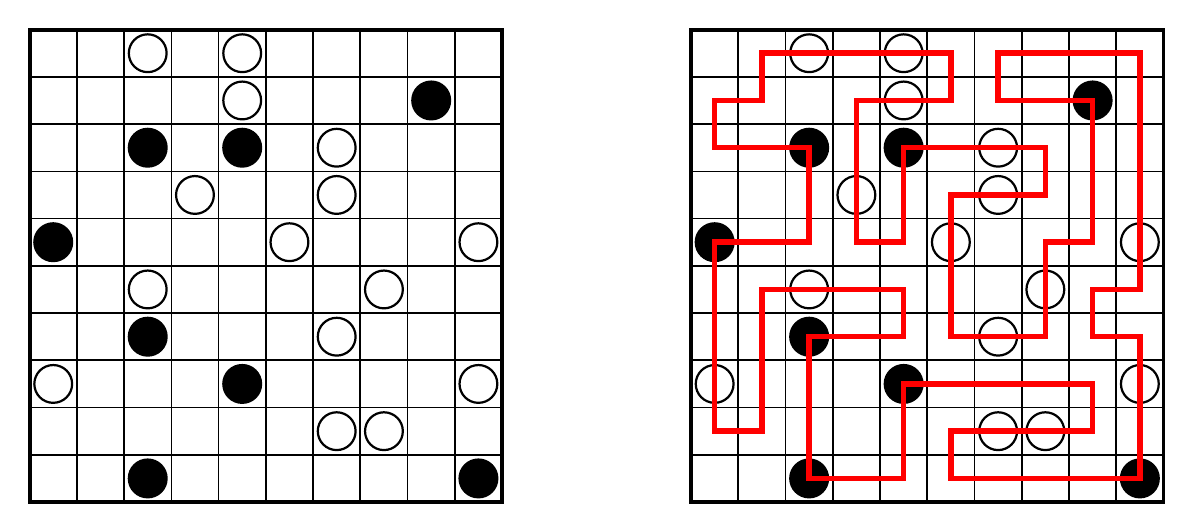
\begin{tikzpicture}[>=latex,thick,scale=0.6]

\def\kreis#1#2{
	\fill[color=#2] #1 circle[radius=0.4];
	\draw #1 circle[radius=0.4];
}

\def\spielfeld{
	\foreach \a in {0.5,1.5,...,8.5}{
		\draw[line width=0.6pt] (-0.5,\a) -- (9.5,\a);
		\draw[line width=0.6pt] (\a,-0.5) -- (\a,9.5);
	}
	\draw[line width=1.4pt] (-0.5,-0.5) rectangle (9.5,9.5);

	\kreis{(2,0)}{black}
	\kreis{(9,0)}{black}

	\kreis{(6,1)}{white}
	\kreis{(7,1)}{white}

	\kreis{(0,2)}{white}
	\kreis{(4,2)}{black}
	\kreis{(9,2)}{white}

	\kreis{(2,3)}{black}
	\kreis{(6,3)}{white}

	\kreis{(2,4)}{white}
	\kreis{(7,4)}{white}

	\kreis{(0,5)}{black}
	\kreis{(5,5)}{white}
	\kreis{(9,5)}{white}

	\kreis{(3,6)}{white}
	\kreis{(6,6)}{white}

	\kreis{(2,7)}{black}
	\kreis{(4,7)}{black}
	\kreis{(6,7)}{white}

	\kreis{(4,8)}{white}
	\kreis{(8,8)}{black}

	\kreis{(2,9)}{white}
	\kreis{(4,9)}{white}
}

\def\pfad{
	\draw[line width=2pt,color=red]
		   (2,0) -- (4,0) -- (4,2) -- (8,2) -- (8,1) -- (5,1)
		-- (5,0) -- (9,0) -- (9,3) -- (8,3) -- (8,4) -- (9,4)
		-- (9,9) -- (6,9) -- (6,8) -- (8,8) -- (8,5) -- (7,5)
		-- (7,3) -- (5,3) -- (5,6) -- (7,6) -- (7,7) -- (4,7)
		-- (4,5) -- (3,5) -- (3,8) -- (5,8) -- (5,9) -- (1,9)
		-- (1,8) -- (0,8) -- (0,7) -- (2,7) -- (2,5) -- (0,5)
		-- (0,1) -- (1,1) -- (1,4) -- (4,4) -- (4,3) -- (2,3)
		-- cycle;
}

\begin{scope}[xshift=-7cm]
	\spielfeld
\end{scope}

\begin{scope}[xshift=7cm]
	\spielfeld
	\pfad
\end{scope}

\end{tikzpicture}
\end{center}
Kann eine nichtdeterministische Turing-Maschine in polynomieller Zeit
entscheiden, ob ein Masyu-Rätsel eine Lösung hat?

\thema{NP}
\thema{polynomieller Verifizierer}

\begin{loesung}
Die Frage ist sicher entscheidbar, indem man alle endlich vielen
möglichen Abfolgen von Feldern daraufhin testet, ob sie Pfade sind
und den vier Bedingungen genügen.
Dafür ist jedoch exponentielle Zeit nötig.

Eine nichtdeterministische Turing-Maschine kann die Frage in polynomieller
Zeit entscheiden, wenn es einen polynomiellen Verifizierer gibt.
Als Zertifikat wird der gesuchte Lösungspfad gefordert, eine Abfolge
von höchstens $n^2$ Feldern.
Damit sind folgende Verifikationen vorzunehmen:
\begin{center}
\begin{tabular}{>{$}c<{$}|p{10cm}|>{$}c<{$}}
\text{Regel}&Verifikation&\text{Laufzeit} \\
\hline
1
&Jedes Feld des Pfades ist ein Nachbarfeld des vorangegangenen Feldes.
&O(n^2)\\
2
&Jedes Element des Pfades mit jedem anderen Element vergleichen,
und kontrollieren, dass alle Elemente verschieden sind.
&O(\frac{n(n-1)}2)\\
3a
&Kontrollieren, ob die Nachbarn eines Feldes mit weissem Kreis
diametral gegenüberliegen.
&O(n^2)\\
3b
&Kontrollieren, ob auf einem der Nachbarfelder eines Feldes mit weissem Kreis
eine $90^\circ$-Abbiegung erfolgt
&O(n^2)\\
4
&Kontrolliere, ob auf jedem Element des Pfades mit einem schwarzen Feld
die Nachbarelemente eine $90^\circ$-Abbiegung bilden.
&O(n^2)\\
\hline
&Total&O(n^2)
\end{tabular}
\end{center}
Damit ist gezeigt, dass der Verifizierer polynomielle Laufzeit hat.
Somit ist Masyu in NP.
\end{loesung}

\begin{diskussion}
Erich Friedmann hat 2002 bewiesen, dass Masyu NP-vollständig ist.
\end{diskussion}

\begin{bewertung}
Entscheidbarkeit ({\bf E}) 1 Punkt,
Prinzip Verifizierer ({\bf V}) 1 Punkt,
Zertifikat spezifiziert ({\bf Z}) 1 Punkt,
Laufzeitschätzung ({\bf L}) 2 Punkte,
Schlussfolgerung polynomieller Verifizierer ({\bf S}) 1 Punkt.
\end{bewertung}






